
\documentclass[journal,UTF8]{IEEEtran}
%\usepackage{ctex}
\usepackage{color}

%
\usepackage{cite}

\ifCLASSINFOpdf
 \usepackage[pdftex]{graphicx}
  % declare the path(s) where your graphic files are
 \graphicspath{{../pdf/}{../jpeg/}}
  % and their extensions so you won't have to specify these with
  % every instance of \includegraphics
\DeclareGraphicsExtensions{.pdf,.jpeg,.png}
\else
  % or other class option (dvipsone, dvipdf, if not using dvips). graphicx
  % will default to the driver specified in the system graphics.cfg if no
  % driver is specified.
\usepackage[dvips]{graphicx}
  % declare the path(s) where your graphic files are
\graphicspath{{../eps/}}
  % and their extensions so you won't have to specify these with
  % every instance of \includegraphics
\DeclareGraphicsExtensions{.eps}
\fi

\usepackage[cmex10]{amsmath}

\usepackage{algorithmic}

\usepackage{array}


\ifCLASSOPTIONcompsoc
  \usepackage[caption=false,font=normalsize,labelfont=sf,textfont=sf]{subfig}
\else
  \usepackage[caption=false,font=footnotesize]{subfig}
\fi

\hyphenation{op-tical net-works semi-conduc-tor}



\begin{document}

\title{An Initial Survey of Artificial Intelligence Approaches to Network Management}

\maketitle

% As a general rule, do not put math, special symbols or citations
% in the abstract or keywords.
% * <karyns@accdon.com> 2017-12-24T08:35:37.488Z:
% 
% General note: Language was unclear in many areas. I have done my best to guess at your intended meaning. Please carefully review all edits. 
% 
% ^.
\begin{abstract}
From my point of view, the artificial intelligence (AI) based network management (NM) could be five classifications: fault, configuration, accounting, performance and security management. In my mind, the next step: write a survey as the start of my research and have a test to understand AI and NM in depth. \textcolor{blue}{After the meeting, we have a better next step that narrowed the network management into flexible industrial automation application integrated with AI and continue to research the state of the art. Meanwhile, we make a simple outline of the topic and find its possibility to apply the European research project together with HDU and other relevant organizations.\footnote{\textcolor{blue}{the blue sentences are the ideas after the meeting.}}}  
 

\end{abstract}

% Note that keywords are not normally used for peerreview papers.
\begin{IEEEkeywords}
Review, Artificial intelligence, Network Management
\end{IEEEkeywords}

% For peer review papers, you can put extra information on the cover
% page as needed:
% \ifCLASSOPTIONpeerreview
% \begin{center} \bfseries EDICS Category: 3-BBND \end{center}
% \fi
%
% For peerreview papers, this IEEEtran command inserts a page break and
% creates the second title. It will be ignored for other modes.
\IEEEpeerreviewmaketitle

\section{Introduction}
For past three weeks, my biggest gain is that I have an overview of AI-based NM although I do not understand all of the papers well after a sample survey of over 50 papers. During this time, the deepest impressions are that at the very early year, even earlier than 1990's, there has been various papers discussing every aspect of network management using AI technologies. To date, definitely, it has become much hotter. The differences are nowadays we use much more complex algorithms and we have much more strong computing ability and much more kinds of application scenarios. 

For AI, when we talk it, in most cases, we mean machine learning. Normally, machine learning is divided into three learning paradigms: supervised, un-supervised and reinforcement learning. When we want to implement some applications. We should also usage some theory or technologies for related paradigm, such as Bayesian theory, Support Vector Machine (SVM), Hidden Markov Model, Q-learning or various kinds of Neural Networks etc. 

Meanwhile, there are various types of communication network appeared in papers: wireless network, cellular network, optical network, IP network, ad hoc network, radio network etc.

Hence, when AI meet NM. We get more concepts, such as machine learning based, AI-based, self-organize (self-configuring, self-healing, self-optimizing and self-protecting), cognitive together with types of network.  

Furthermore, lots of labs are focusing on these concepts. Table \ref{table:Labs} shows the information of part of the labs. To my best knowledge, it is ranked by importance and of course, it is not complete. I will continuously update this survey.

\begin{table*}
	\scriptsize \caption{Information of labs working on AI-based NM}
	\label{table:Labs}
	\begin{center}
		\renewcommand{\arraystretch}{1.4}
		\setlength\tabcolsep{3pt}
		\begin{tabular}{|l|c|c|c|c|c|}
			\hline
			Head&Country& University &Personal Articles& collected papers  & key words\\
			\hline
			R. Boutaba &Canada &University of Waterloo&199  & 2      &       \\
			\hline
			Honggang Zhang & China & Zhejiang University&190  & 7  &       \\
            \hline
 			Hanzo Lajos  & UK  & University of Southampton&1216 & 2  &       \\
            \hline  
 			Petri Mähönen&Germany&RWTH Aachen University&235 & 1& \\
            \hline  
 			P. Venkataram P&India&Indian Institute of Science&143 & 2& \\
            \hline 
 			Xiangming Wen&China& Beijing University of Posts and Telecommunications &210& 2  &       \\
            \hline  
 			Qadir J.&Pakistan&National University of Sciences and Technology&67&1& \\
            \hline         
		\end{tabular}
	\end{center}
\end{table*}

As the most important thing, the classification of NM direction is defined differently by different researchers.

Kumar, et al. \cite{Kumar1997Artificial}, in 1997 a very early year, give an overview of the AI in NM which is classified into \textbf{fault management, configuration management, accounting management, performance management, security management} but more expert system than AI technologies are discussed. 20 years later, \cite{Ayoubi2018Machine} from University of Waterloo describes the overview of machine learning as the same classifications meanwhile they have explained more machine learning technologies and provided an impressive framework named C-MAPE (Cognitive-Monitor-Analyze-Plan-Execute over a shared Knowledge) in FIG.\ref{fig:CMAPE}. This kind of classifications comes from \textbf{Telecommunications Management Network (TMN) Recommendations} \cite{ITU1992TMN}.

Then, in \cite{Boutaba2018A}, Boutaba, et al. have a much more comprehensive discussion of machine learning on networking which has over 500 citations. It contains 8 directions: \textbf{traffic prediction, traffic classification, traffic routing, congestion control, resource management, fault management, QoS and QoE management, network security} and each direction has its subsections, illustrated in FIG. \ref{fig:MLinN}. 



Li Rongpeng, et al. \cite{Li2017Intelligent} presents the AI int context of 5G and have a different view of the classifications which are \textbf{radio resource management, mobility management, management and orchestration, service provisioning management}.

Jiang and Hanzo Lajos in \cite{Jiang2017Machine} also provides a machine learning paradigms in 5G shown in FIG. \ref{fig:MLin5G}. They distinguish the applications as the type of machine learning.

Then, under the guide of these survey, I read some papers simply and when I have a look of a paper, I will record something to its related section below. 
%Qi, et al. \cite{Qi2007Artificial} provides us a comprehensive discussion in network management.

\begin{figure}
	\centering
	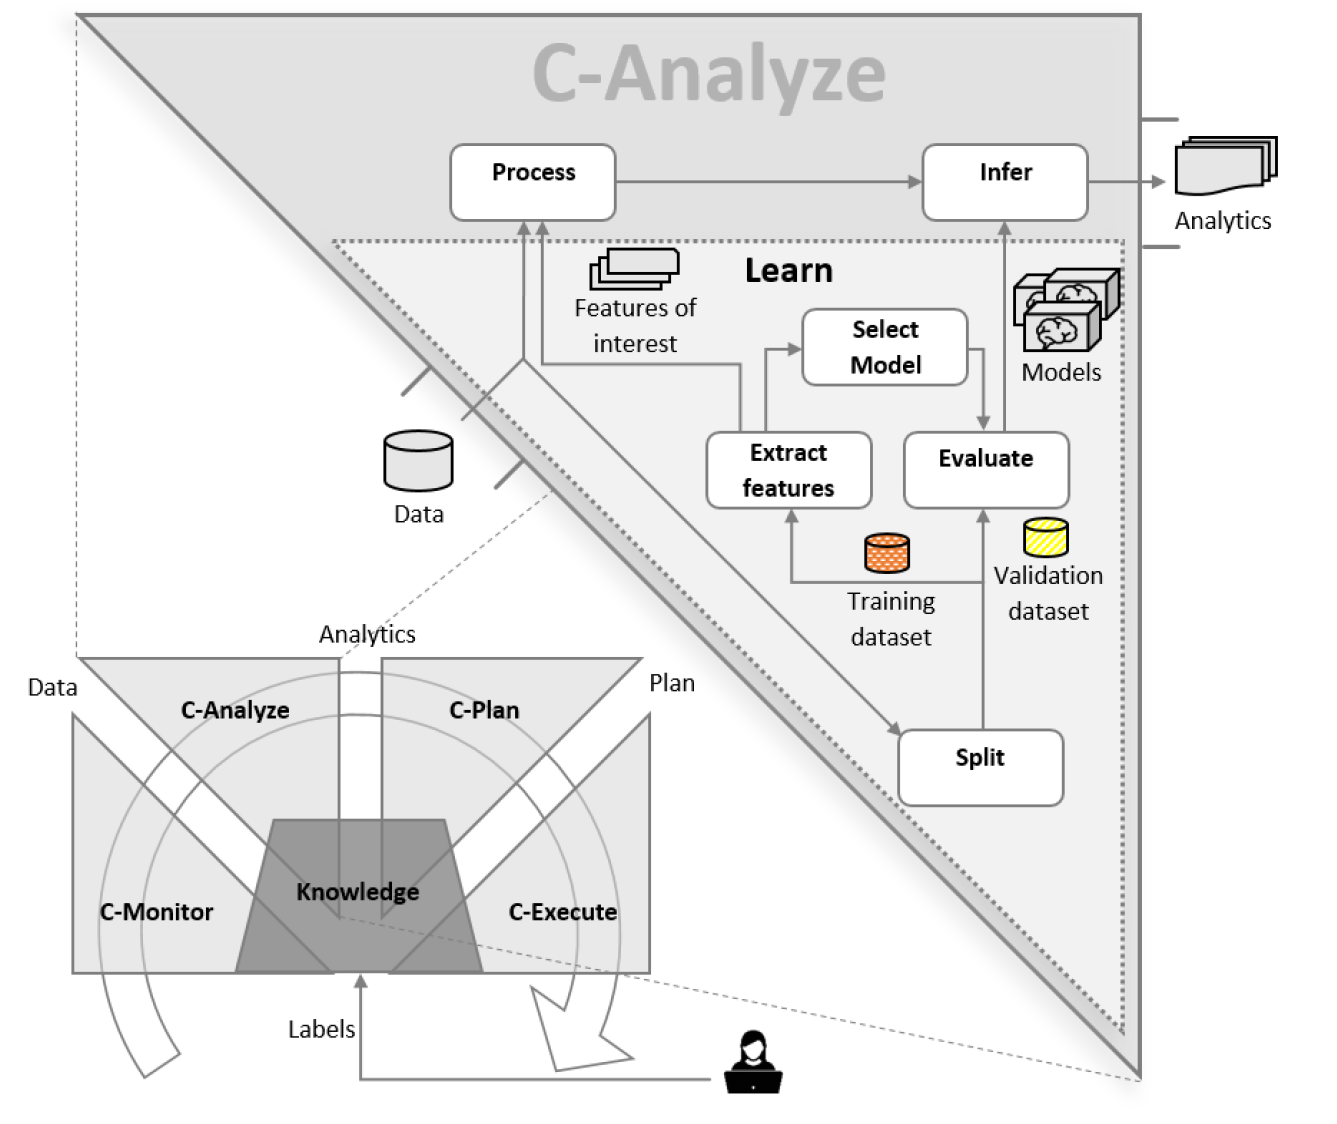
\includegraphics[width=3in]{fig/C-MAPE.png}
	\caption{C-MAPE.}
	\label{fig:CMAPE}
\end{figure}

\begin{figure*}
	\centering
	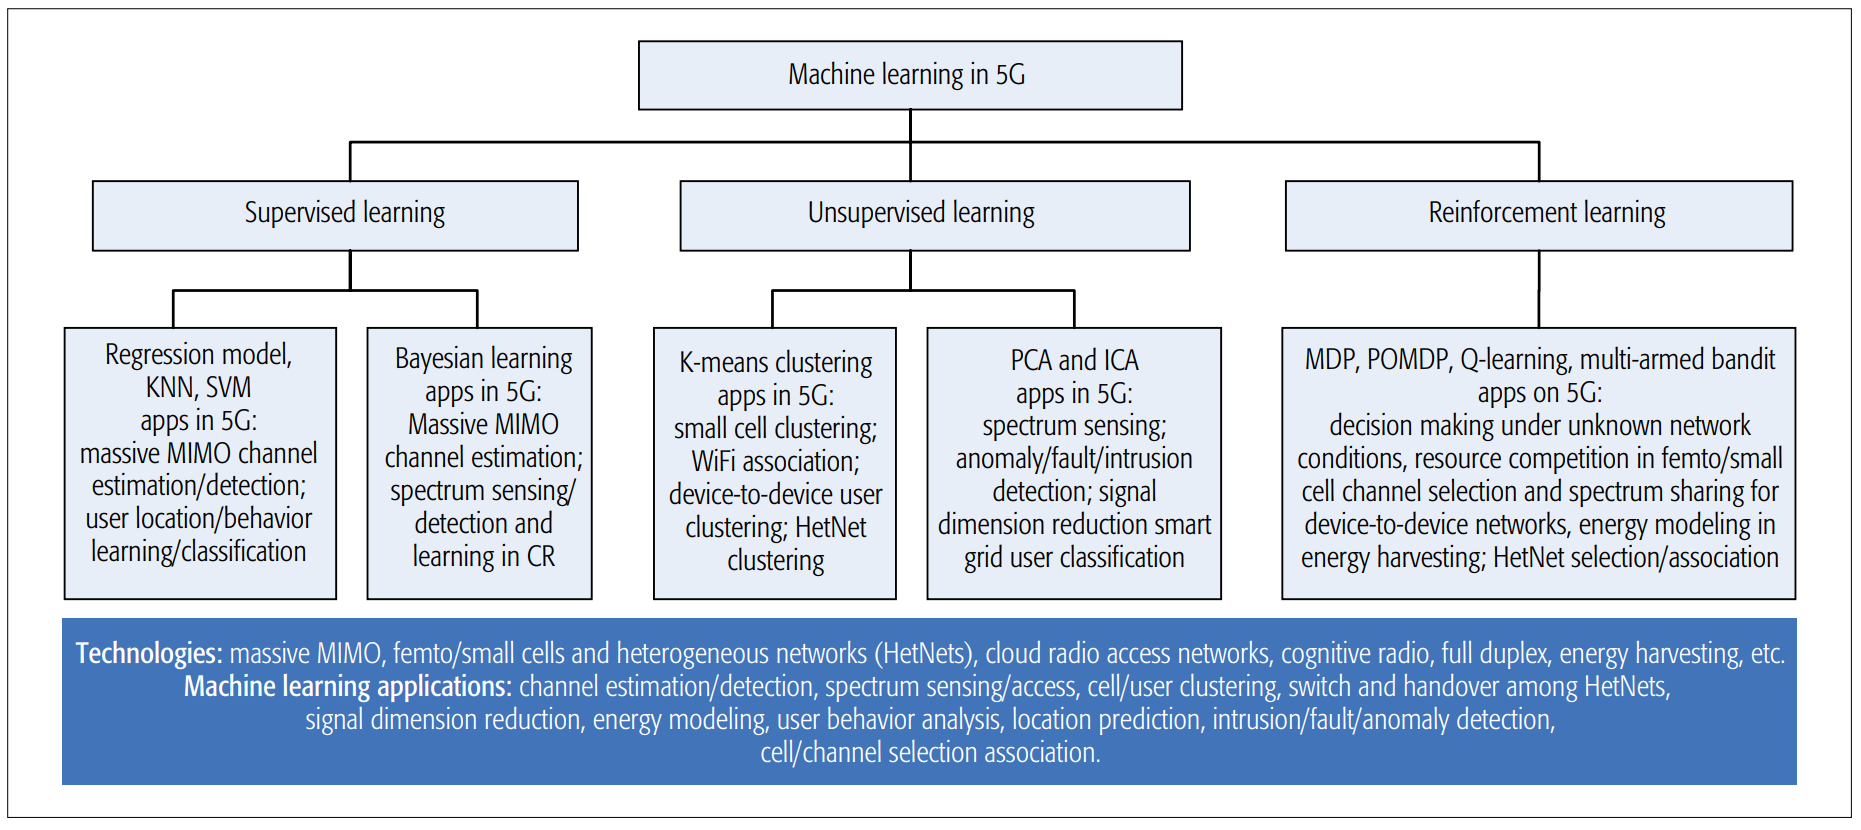
\includegraphics[width=7in]{fig/MLin5G.png}
	\caption{Machine Learning in 5G.}
	\label{fig:MLin5G}
\end{figure*}

 \begin{figure*}
	\centering
	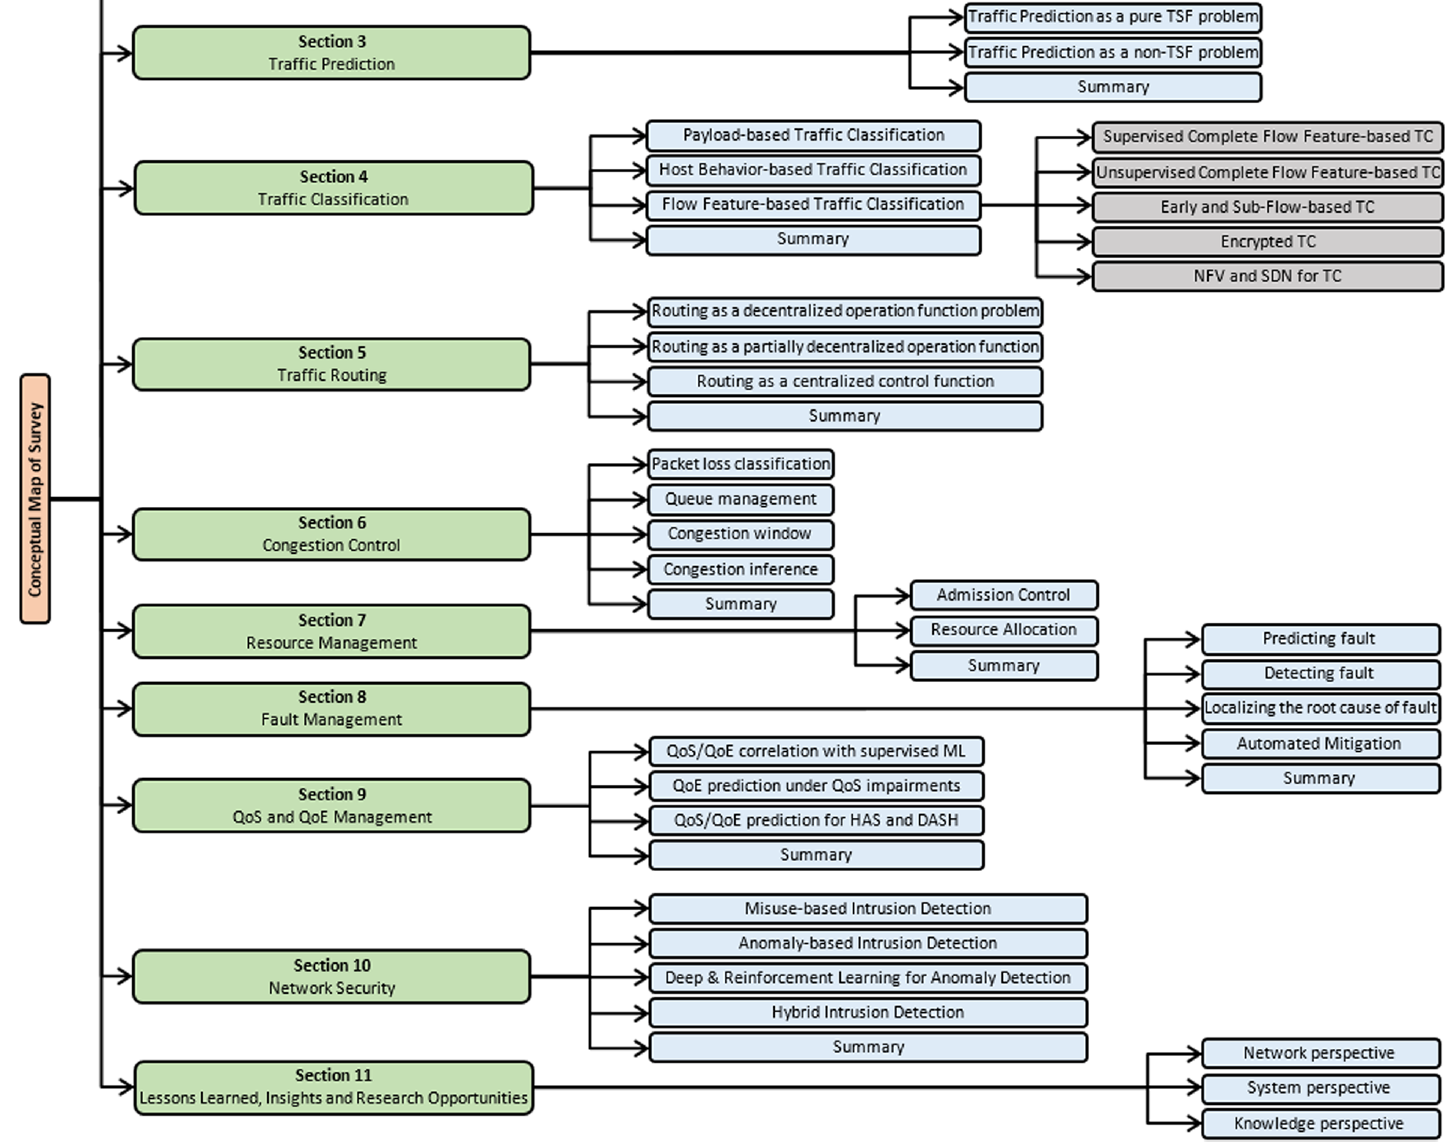
\includegraphics{fig/MLinN.png}
	\caption{Machine Learning in Networking}
	\label{fig:MLinN}
\end{figure*}


\section{Overview of AI}
\subsection{Supervised Learning}

\subsection{Un-supervised Learning}

\subsection{Reinforcement Learning}
\section{Overview of NM}
\subsection{Traffic Classification}
\cite{Williams2006A} is a review of traffic classification. Then a lot of papers\cite{Jin2012A,Huang2012On,Soysal2010Machine} discuss about it.
\subsection{Traffic Prediction}
\cite{Hua2017Traffic} from Zhejiang University is about traffic prediction.
\subsection{Traffic Routing}
Qadir\cite{Qadir2016Artificial} from Pakistan gaves us a review about congnitive routing.

\cite{Hui2002Reinforcement}, \cite{Saleem2017Clustering}



\subsection{Mobility Management}
\cite{Cao2017AIF} poses a AI framework for wireless NM which is used in a case of mobility management, where a ping-pong problem is addressed.  

\subsection{Resource management}
\cite{Morozs2016Cognitive,L2017Primary} are about spectrum management.

\subsection{Fault Management}

The key elements in fault management are: fault prevention, fault detection, fault localization and isolation, fault repair and restoration.

\cite{Maxion1990Anomaly} is a very early paper using machine learning without specify of it.

\cite{Hood1997Proactive} uses the log data to train the Bayesian network for fault detection and provides  a wired office network

\cite{Ding2004Predictive} presents a dynamic Bayesian Network for large IP network which improves the problem of \cite{Hood1997Proactive} that dynamically evolve over time.

\cite{Snow2005Assessing} poses a limited method of NN to estimate the dependability of a 2G wireless network.


\cite{Kogeda2006A}, \cite{Lu2010Using} 

\cite{pellegrini2015machine} is a framework of machine learning.

\cite{Song2017Failure} poses a ML method based on physical indicates in optical networks.

\cite{Kumar2017Fault}



Fault detection
\cite{baras1997automated} is a early paper discussing fault detection using NN.

\cite{Rao2006Operational} propses a method of Operational Fault Detection whose fault or alarm thresholds are determined by learning expected deviations during a training phase.

\cite{Qader2017Comparative} build a real-time fault detection and classification model.

\cite{Qader2014Fault} select 12 features  and use the traffic patterns to form clusters that represent normal traffic, link failure, server crash, broadcast storm and protocol error.


\cite{Moustapha2008Wireless} detect faulty nodes in a WSN using RNN.

\cite{Hajji2005Statistical}  propose an unsupervised fault detection mechanism.

\cite{Hashmi2017Enabling} use different unsupervised algorithms to detect faults in a broadband service provider network that serves about 1.3 million customers.


\cite{Rafique2018Cognitive}

\subsection{Performance management}
\cite{Kumar2002Network} used the RL to turning the management when performance degradation occurs. From my point of view, it have used the DQL (Deep Q-learning).

\subsection{Security Management}

\cite{Zheng2016Cognitive,J2018AI}





\subsection{Service Management}
\cite{Rovcanin2015Experimental} uses a reinforcement learning approach to optimize service.

\cite{Zhao2018Deep,Xianfu2018Multi} presents reinforcement approachs to service slicing. 

\subsection{Platform}
\cite{Ren2018Low} pose a platform of AI-based NM.


\section{A Case of Reinforcement Learning}



\section{Conclusion}
\label{conclusion}
After having a look of these papers, I strongly agree with the 5-type classification: \textbf{fault, configuration, accounting, performance and security management}. I think fault, performance and accounting management are three stages of NM. Configuration and security management effect throughout the NM. 

Since the past papers are too much of all 5 classifications, I think I must narrow my topic into one of them firstly. 

If I should select one from the 5, the fault management would be better. Because it is the first step of NM. However, several questions are still confused me. Firstly, to my best knowledge, as far as I know, lots of work also have been done on fault management. Maybe if we further narrow it to industry or automation then the situation maybe changed. On the other hand, I want my topic which would be usable to some further projects and could be studied for a long time, not just limited to PhD study and could be based on ifak's past research. From my point of view, these three points are important but I do not know how to deal with it. Additionally, if fault management is the topic, is it relatively a little bit easier to do some experiment or have some implementations later. \textcolor{blue}{After the meeting, most of the confusions are clarified.} 

If the topic has an initial decision. For the next stage, I plan to do two things.
\begin{enumerate}
	\item Write a survey of my topic as the beginning of my research and hopefully it will be published in a journal.
	\item Have a test of wireless AI which will let me know both NM and AI in depth.
\end{enumerate}

\textcolor{blue}{After the meeting, since the network management could be narrowed into flexible industrial automation application, we have the new next step:
\begin{enumerate}
	\item Continue to research the state of the art and make a simple outline of the topic.
	\item Find the possibility to apply the European research project together with HDU and the application deadline of the possible European project is 2019.3.  
\end{enumerate}}


\ifCLASSOPTIONcaptionsoff
  \newpage
\fi



% trigger a \newpage just before the given reference
% number - used to balance the columns on the last page
% adjust value as needed - may need to be readjusted if
% the document is modified later
%\IEEEtriggeratref{8}
% The "triggered" command can be changed if desired:
%\IEEEtriggercmd{\enlargethispage{-5in}}

% references section

% can use a bibliography generated by BibTeX as a .bbl file
% BibTeX documentation can be easily obtained at:
% http://www.ctan.org/tex-archive/biblio/bibtex/contrib/doc/
% The IEEEtran BibTeX style support page is at:
% http://www.michaelshell.org/tex/ieeetran/bibtex/
%\bibliographystyle{IEEEtran}
% argument is your BibTeX string definitions and bibliography database(s)
%\bibliography{IEEEabrv,../bib/paper}
%
% <OR> manually copy in the resultant .bbl file
% set second argument of \begin to the number of references
% (used to reserve space for the reference number labels box)

\bibliographystyle{IEEEtran}
\bibliography{reference}

% biography section
%
% If you have an EPS/PDF photo (graphicx package needed) extra braces are
% needed around the contents of the optional argument to biography to prevent
% the LaTeX parser from getting confused when it sees the complicated
% \includegraphics command within an optional argument. (You could create
% your own custom macro containing the \includegraphics command to make things
% simpler here.)
%\begin{IEEEbiography}[{\includegraphics[width=1in,height=1.25in,clip,keepaspectratio]{mshell}}]{Michael Shell}
% or if you just want to reserve a space for a photo:

%\begin{IEEEbiography}[{\includegraphics[width=1in,height=1.25in,clip,keepaspectratio]{fig/Author_HuifengWu.eps}}]{Huifeng Wu} received the Ph.D. degree in computer science and technology from Zhejiang university, Hangzhou, China, in 2006. He is currently a professor in the institute of intelligent and software Technology, Hangzhou Dianzi University. His research interests include software development methods and tools, software architecture, embedded system, intelligent control \& automation.
%	
%\end{IEEEbiography}
%\begin{IEEEbiography}[{\includegraphics[width=1in,height=1.25in,clip,keepaspectratio]{fig/Author_YiYan.eps}}]{Yi Yan} received B.S. in automatic control engineering form Zhejiang Sci-Tech University in 1984, M.S. in computer engineering from Beijing University of Postal Telecommunications in 1990. Currently he is the director and full professor in institute of intelligent and software Technology, Hangzhou Dianzi University. His research interests include embedded system, advanced manufacturing system, intelligent control \& automation, and intelligent instruments.
%	
%	
%\end{IEEEbiography}
%\begin{IEEEbiography}[{\includegraphics[width=1in,height=1.25in,clip,keepaspectratio]{fig/Author_DanfengSun.eps}}]{Danfeng Sun} received M.S. in computer architecture from Hangzhou DianZi University in 2011. He is currently a research assistant in the Institute of Industrial Internet, Hangzhou DianZi University. His research interests include embeded system, motion control and IIoT.
%\end{IEEEbiography}
%\begin{IEEEbiography}[{\includegraphics[width=1in,height=1.25in,keepaspectratio,angle=-90]{fig/Author_ReneSimon.eps}}]{Rene Simon} obtained a doctor of engineering at the Otto-von-Guericke University Magdeburg in 2001. He is Professor of Control Systems at the Department of Automation and Computer Sciences, Harz University of Applied Sciences, Wernigerode, Germany. His major research fields include engineering of automation systems, especially industrial controllers. He is chairman of PLCopen and project leader IEC 61131-10 Ed. 1.0.
%\end{IEEEbiography}



% insert where needed to balance the two columns on the last page with
% biographies
%\newpage


% You can push biographies down or up by placing
% a \vfill before or after them. The appropriate
% use of \vfill depends on what kind of text is
% on the last page and whether or not the columns
% are being equalized.

%\vfill

% Can be used to pull up biographies so that the bottom of the last one
% is flush with the other column.
%\enlargethispage{-5in}



% that's all folks
\end{document}


